\documentclass[a4paper,11pt]{scrartcl}

\usepackage[margin=2.cm]{geometry}

\usepackage[english]{babel}
\usepackage[utf8]{inputenc}

\usepackage[pdftex]{graphicx}

\usepackage{amsmath}
\usepackage{amssymb}

\usepackage{dsfont}

\usepackage{hyperref}

\newcommand{\exd}{\mathbf{d}}
\newcommand{\excod}{\exd^{*}} %or \delta
\newcommand{\Div}{\text{Div}}
\newcommand{\Rot}{\text{Rot}}

\newcommand{\R}{\mathds{R}}


% IDENTIFIERS for math mode:

%surface (manifold) -> M, S, \Omega 
\newcommand{\M}{M}
%volume element (volume measure) -> \mu, dA, d\Omega
\newcommand{\dA}{dA}
%director field (contra-vector)
\newcommand{\p}{\mathbf{p}}
\newcommand{\q}{\mathbf{q}}
%director field (co-vector, flat of contra-vector)
\newcommand{\pfl}{\mathbf{p}^{\flat}}
\newcommand{\qfl}{\mathbf{q}^{\flat}}
%discrete director field (co-vector, flat of contra-vector)
\newcommand{\pflh}{\mathbf{p}^{\flat}_{h}}
\newcommand{\pflhOld}{\widehat{\mathbf{p}}^{\flat}_{h}}
\newcommand{\qflh}{\mathbf{q}^{\flat}_{h}}
%discrete director field (contra-vector)
\newcommand{\ph}{\mathbf{p}_{h}}
%discrete PD director field (co-vector, flat of contra-vector)
\newcommand{\PDpflh}{\underline{\mathbf{p}}^{\flat}_{h}}
\newcommand{\PDqflh}{\underline{\mathbf{q}}^{\flat}_{h}}
%discrete director field (contra-vector)
\newcommand{\PDph}{\underline{\mathbf{p}}_{h}}
\newcommand{\PDqh}{\underline{\mathbf{q}}_{h}}
%discrete PD director field OLD SOLUTION (co-vector, flat of contra-vector)
\newcommand{\PDpflhOld}{\underline{\widehat{\mathbf{p}}}^{\flat}_{h}}
%discrete director field OLD SOLUTION (contra-vector)
\newcommand{\PDphOld}{\underline{\widehat{\mathbf{p}}}_{h}}
%Frank Oseen Energy (without Lagrange term for normalizing)
\newcommand{\EOS}{E_{\text{FO}}}
%Normalizing energy
\newcommand{\EN}{E_{n}}
%Laplace-Beltrami or Rot-Rot-Laplace
\newcommand{\LB}{\boldsymbol{\Delta}^{\text{\tiny RR}}}
%Laplace-CoBeltrami or Grad-Div-Laplace
\newcommand{\LCB}{\boldsymbol{\Delta}^{\text{\tiny GD}}}
%Laplace-deRham
\newcommand{\LDR}{\boldsymbol{\Delta}^{\text{\tiny dR}}}
%discrete Laplace-Beltrami or Rot-Rot-Laplace
\newcommand{\LBh}{\LB_{h}}
%Laplace-CoBeltrami or Grad-Div-Laplace
\newcommand{\LCBh}{\LCB_{h}}
%Laplace-deRham
\newcommand{\LDRh}{\LDR_{h}}
%Landau symbol
\renewcommand{\O}{\mathcal{O}}
%Vertices
\newcommand{\V}{\mathcal{V}}
%Edges
\newcommand{\E}{\mathcal{E}}
%Faces
\newcommand{\F}{\mathcal{F}}
%edge vector
\newcommand{\e}{\mathbf{e}}
%vertex vector
\renewcommand{\v}{\mathbf{v}}
%PD-Basis
\newcommand{\PDxi}{\boldsymbol{\xi}}



\begin{document}

\tableofcontents

\section{Frank Oseen energy}

In \( \R^{3} \):
\begin{align}\label{eqFO1}
  \EOS = \frac{1}{2}\int_{\Omega} K_{1}\left( \nabla\cdot\p \right)^{2} 
                        + K_{2}\left( \p\cdot\left[ \nabla\times\p \right] \right)^{2}
                        + K_{3}\left\| \p\times\left[ \nabla\times\p \right] \right\|^{2} dV
\end{align}
With the Langrange identity for the \( K_{3} \)-term, we cann rewrite \eqref{eqFO1} to
\begin{align}\label{eqFO2}
  \EOS = \frac{1}{2}\int_{\Omega} K_{1}\left( \nabla\cdot\p \right)^{2} 
                        + (K_{2}-K_{3})\left( \p\cdot\left[ \nabla\times\p \right] \right)^{2}
                        + K_{3}\left\| \p \right\|^{2}\left\| \nabla\times\p \right\|^{2} dV
\end{align}
If we restrict \eqref{eqFO2} to a 2-dimensional Manifold \( \M\subset\Omega \) 
and postulate that \( \p\in T_{X}\M \) is a normalized tangential vector in \( X\in\M \), we get
\begin{align}
  \EOS = \frac{1}{2} \int_{\M} K_{1}\left( \Div\p \right)^{2} + K_{3}\left( \Rot \p \right)^{2} \dA 
\end{align}
In terms of exterior calculus with the corresponding 1-form \( \pfl\in\Lambda^{1}(M) \), 
,i.e. \( \left( \pfl \right)^{\sharp} = \p\), we obtain
\begin{align}
  \EOS = \frac{1}{2} \int_{\M} K_{1}\left( \excod\pfl \right)^{2} + K_{3}\left( *\exd \pfl \right)^{2} \dA
\end{align}
where the exterior coderivative \( \excod := -* \exd * \) is the \( L^{2} \)-orthogonal operator of the exterior derivative \( \exd \). 
(Note \( \Div\p = -\excod\pfl \) and \( \Rot\p = *\exd\pfl \)) 

  \subsection{Functional derivative}
  
  With the  \( L^{2} \)-orthogonality of the exterior derivative and coderivative 
  (\( \left\langle \exd\bullet, \bullet  \right\rangle_{L^{2}} = \left\langle \bullet,\excod\bullet \right\rangle_{L^{2}} \))
  and a arbitrary \( \alpha\in\Lambda^{1}(M) \) we get
  \begin{align}
    \int_{\M} \left\langle\frac{\delta\EOS}{\delta\pfl} , \alpha \right\rangle \dA
      &= \lim_{\epsilon\rightarrow 0} \frac{1}{\epsilon}\left( \EOS\left[ \pfl + \epsilon\alpha \right] - \EOS\left[ \pfl\right]\right) \\
      &=  \lim_{\epsilon\rightarrow 0} \frac{1}{2\epsilon} \int_{\M} 
                K_{1}\left( 2\epsilon \left( \excod\pfl \right)\left( \excod\alpha \right) 
                            + \epsilon^{2}\left( \excod\alpha \right)^{2} \right) \\
      &\phantom{= \lim_{\epsilon\rightarrow 0} \frac{1}{2\epsilon} \int_{\M}}
                +K_{3}\left(2\epsilon\left\langle \exd\pfl, \exd\alpha \right\rangle
                            + \epsilon^{2}\left\| \exd\alpha \right\|^{2}\right)\dA \\
      &= -\int_{\M} K_{1} \left\langle \LCB\pfl, \alpha \right\rangle + K_{3} \left\langle \LB\pfl, \alpha \right\rangle \dA \\
      &= \int_{\M} \left\langle -\left( K_{1}\LCB + K_{3}\LB\right)\pfl , \alpha \right\rangle \dA
  \end{align}
  where \( \LB = -\excod\exd = *\exd *\exd  \) is the Vector-Laplace-Beltrami-Operator or Rot-Rot-Laplace 
  and \( \LCB = - \exd\excod = \exd * \exd * \) is the Vector-Laplace-CoBeltrami-Operator or Grad-Div-Laplace.
  Hence, for a One-Constant-Approximation \( K_{1} = K_{3} =: K_{0} \), we obtain
  \begin{align}
    \int_{\M} \left\langle\frac{\delta\EOS}{\delta\pfl} , \alpha \right\rangle \dA
     &= \int_{\M} \left\langle K_{0}\LDR\pfl , \alpha \right\rangle \dA
  \end{align}
  where \( \LDR = -\LB - \LCB = \excod\exd + \exd\excod\) is the Laplace-de Rham operator.
  
  \subsection{Unit vector invariance}
  
  If \( \p\in T_{X}\M \) is a unit vector on \( \M \), we can describe all unit vectors \(  \) in \( X\in\M \) as a rotation in the tangential space
  with angle \( \phi\in\R \):
  \begin{align}
    \q = \cos\phi\p + \sin\phi\left( *\p \right)
  \end{align}
  \( *\p = \left( *\pfl \right)^{\sharp}\) is the Hodge dual of \( \p \), i.e. a quarter rotation of \( \p \). 
  For a space independent angle \( \phi \), i.e. \( \exd\phi=0 \), straight forward calculations implies
  \begin{align}
     \left\| \Rot (*\p) \right\| &=  \left\| *\exd*\pfl \right\| = \left\| \Div\p \right\|\\
     \left\| \Div (*\p) \right\| &= \left\| *\exd**\pfl  \right\| = \left\| *\exd\pfl  \right\| = \left\|\Rot\p\right\|\\ 
     \left\| \Rot\q \right\|^{2} &= \left\| *\exd\qfl \right\|^{2} = \left\| \exd\qfl \right\|^{2} \\
                                      &=  \cos^{2}\phi\left\| \Rot\p \right\|^{2} 
                                        + \sin^{2}\phi\left\| \Div\p \right\|^{2}
                                        + 2\cos\phi\sin\phi\left\langle \exd\pfl, \exd * \pfl \right\rangle\\
    \left\| \Div\q \right\|^{2} &= \left\| *\exd*\qfl \right\|^{2} = \left\| \exd*\qfl \right\|^{2}\\
                                     &= \cos^{2}\phi\left\| \Div\p \right\|^{2} 
                                        + \sin^{2}\phi\left\| \Rot\p \right\|^{2}
                                        - 2\cos\phi\sin\phi\left\langle \exd\pfl, \exd * \pfl \right\rangle  
  \end{align}
  Finally, we get for the One-Constant-Approximation of the Frank-Oseen-Energy
  \begin{align}
    \EOS[\q] = \EOS[\p]
  \end{align}


\section{Normalizing energy}

To constrain \( \p \) is normalized, we add
\begin{align}
  \EN = \int_{\M} \frac{K_{n}}{4} \left( \left\| \p \right\|^{2} - 1 \right)^{2} \dA
\end{align}
to the Frank Oseen energy.
Note that the norm defined by the metric \( g \) on the manifold \( \M \) is invariant regarding lowering or rising the indices, i.e.
\begin{align}
  \left\| \p \right\|^{2} = p^{i}g_{ij}p^{j} = p_{i} g^{ij} p_{j} = \left\| \pfl \right\|^{2}
\end{align}

  \subsection{Functional derivative}

  By variating \( \pfl \) under the norm with an arbitrary \( \alpha\in\Lambda^{1}(\M) \), we obtain
  \begin{align}
    \left\| \pfl + \epsilon \alpha \right\|^{2} &= \left\| \pfl \right\|^{2} 
                                                  + 2\epsilon\left\langle \pfl, \alpha \right\rangle
                                                  + \epsilon^{2}\left\| \alpha \right\|^{2}
  \end{align}
  If we are only interesting in linear terms (in \( \epsilon \)), this leads to
  \begin{align}
    \left( \left\| \pfl + \epsilon \alpha \right\|^{2} - 1 \right)^{2}
            &= \left( \left\| \pfl \right\|^{2} - 1  + 2\epsilon\left\langle \pfl, \alpha \right\rangle 
                  + \O\left( \epsilon^{2} \right) \right)^{2}\\
            &= \left( \left\| \pfl \right\|^{2} - 1 \right)^{2} 
                + 4\epsilon\left(\left\| \pfl \right\|^{2} - 1 \right)\left\langle \pfl, \alpha \right\rangle
                + \O\left( \epsilon^{2} \right)
  \end{align}
  Hence, we get for the functional derivative of \( \EN \)
  \begin{align}
    \int_{\M} \left\langle\frac{\delta\EN}{\delta\pfl} , \alpha \right\rangle \dA
      &= \lim_{\epsilon\rightarrow 0} \frac{1}{\epsilon}\left( \EN\left[ \pfl + \epsilon\alpha \right] - \EN\left[ \pfl\right]\right) \\
      &= \int_{\M} \left\langle K_{n} \left( \left\| \pfl \right\|^{2} - 1 \right)\pfl , \alpha \right\rangle \dA
  \end{align}


\section{Model equations}
  To minimize the energy \( E := \EOS + \EN \) we choose a time evolving approach. 
  Hence, with the fundamental lemma of calculus of variations, we will use the time depended differential equation in terms of exterior
  calculus
  \begin{align} \label{eqPOC}
    \partial_{t}\pfl = -\frac{\delta E}{\delta\pfl}
                     = -K_{0}\LDR\pfl - K_{n} \left( \left\| \pfl \right\|^{2} - 1 \right)\pfl
  \end{align}
  or in general, if we don't want to use the One-Constant-Approximation,
  \begin{align} \label{eqP}
    \partial_{t}\pfl = \left( K_{1}\LCB + K_{3}\LB\right)\pfl - K_{n} \left( \left\| \pfl \right\|^{2} - 1 \right)\pfl
  \end{align}
  Note that if we apply the Hodge operator on the whole equations, we get the Hodge dual equations
  \begin{align}
    \label{eqDOC}
    \partial_{t}(*\pfl) &= -K_{0}\LDR (*\pfl) - K_{n} \left( \left\| \pfl \right\|^{2} - 1 \right)(*\pfl) \\
    \label{eqD}
                        &=  \left( K_{1}\LB + K_{3}\LCB\right) (*\pfl) - K_{n} \left( \left\| \pfl \right\|^{2} - 1 \right)(*\pfl)
  \end{align}
  which are very useful for the DEC discretization later in context.
  But this leads to pay attention, because only in the first line (One-Constant-Approximation) we see, 
  that the Hodge dual equations in \( *\pfl \) is the same as the primal equation in \( \pfl \). 
  In the general case (second line), we must "swap" the Laplace operators.



\section{Needed DEC stuff}
  
For further information see for example \cite{whitney,hirani}. 

  \subsection{Surface Mesh}
    ...wellcentered manifoldlike simplicial complex, bla, bla, blub...

  \subsection{Discrete 1-forms}

  The main concept to represent a discrete 1-form \( \pflh\in\Lambda_{h}^{1}(K) \) is to approximate the contraction of the continuous 1-Form 
  \( \pfl\in\Lambda^{1}(M) \) on all edges \( e\in\E \)
  \begin{align}
    \pflh(e) := \int_{\pi(e)}\pfl \approx \int_{0}^{1} \pfl_{X_{e}(\tau)}\left( \dot{X}_{e}(t) \right) dt = \pfl_{X_{e}(\tau)}(\e)
  \end{align}
  where \( \pi:K\rightarrow \M \) is the glueing map, who project the elements of the surface mesh to the manifold.
  \( X_{e}(t) = t\v_{2} + (1-t)\v_{1} \) is the linear barycentric parametrisation of the edge \( e=\left[ v_{1}, v_{2} \right]\).
  The existence of a intermediate value \( \tau\in\left[ 0,1 \right] \), so that \( \e\in T_{X_{e}(\tau)}M \),
  is ensured by the mean value theorem.
  Other discrete forms of arbitrary degree and theirs hodge duals can be interpreted in a similarly way.

  \subsection{Discrete Laplace operators}
    
    In the discrete exterior calculus discrete Operators are defined by successively interpretation of the basic operations on the forms, 
    like the Hodge operator \( * \) or the exterior derivative \( \exd \), as geometric operators on the simplices, 
    like the Voronoi dual operator \( \star \) or the boundary operator \( \partial \) (see \cite{hirani}).
    This results for example to a discrete definition of \( \LB \) for a discrete 1-form \( \pflh\in\Lambda^{1}_{h}(M) \) on a edge 
    \(e\in\E \)
    \begin{align}
      \LBh\pflh(e) &:=  \left(*\exd*\exd \pflh\right)(e)
                     = -\frac{\left| e \right|}{\left| \star e \right|} \left(\exd * \exd  \pflh\right)(\star e) \\
                    &=  -\frac{\left| e \right|}{\left| \star e \right|} \left(* \exd  \pflh\right)(\partial\star e)
                     = -\frac{\left| e \right|}{\left| \star e \right|} \sum_{f\succ e} s_{f,e} \left(* \exd \pflh\right) (\star f) \\
                    &= -\frac{\left| e \right|}{\left| \star e \right|} \sum_{f\succ e} \frac{s_{f,e}}{\left| f \right|} 
                                \left(\exd\pflh\right)(f)
                     = -\frac{\left| e \right|}{\left| \star e \right|} \sum_{f\succ e} \frac{s_{f,e}}{\left| f \right|} \pflh(\partial f)\\
                    &= -\frac{\left| e \right|}{\left| \star e \right|} \sum_{f\succ e} \frac{s_{f,e}}{\left| f \right|}
                                \sum_{\tilde{e}\prec f} s_{f,\tilde{e}} \pflh(\tilde{e})
    \end{align}
    or for \( \LCB \)
    \begin{align}
      \LCBh\pflh(e) &:= \left( \exd * \exd * \pflh\right) (e)
                      = \left( * \exd *\pflh \right) (\partial e) \\
                     &= \sum_{v\prec e} s_{v,e} \left( * \exd * \pflh \right)(v) 
                      = \sum_{v\prec e} \frac{s_{v,e}}{\left| \star v \right|} \left( \exd * \pflh \right)(\star v)\\
                     &= \sum_{v\prec e} \frac{s_{v,e}}{\left| \star v \right|} \left( * \pflh \right)(\partial\star v)
                      = -\sum_{v\prec e} \frac{s_{v,e}}{\left| \star v \right|} \sum_{\tilde{e}\succ v}
                                s_{v,\tilde{e}} \left( * \pflh \right) (\star \tilde{e}) \\
                     &= -\sum_{v\prec e} \frac{s_{v,e}}{\left| \star v \right|} \sum_{\tilde{e}\succ v}
                                s_{v,\tilde{e}} \frac{\left| \star\tilde{e} \right|}{\left| \tilde{e} \right|}\pflh(\tilde{e})
    \end{align}
    where the sign \( s_{f,e} \) is +1 if the face \( f\succ e \) is in the left of the edge \( e \) (-1 otherwise)
    and \( s_{v,e} \) is +1 if the edge \( e\succ v \) points to the vertex \( v \) and -1 if \( e \) points away from \( v \)
    (see figure \ref{figSigns}).
    We see \( \LBh \), \( \LCBh \) and also \( \LDRh := -\LBh -\LCBh \) are linear operators in \( \pflh(\tilde{e}) \)
    and therefor results in sparse matrices if the \( \pflh(\tilde{e}) \) are our degree of freedoms.
    \begin{figure}
      \begin{minipage}[htp]{.25\textwidth}
        \centering
        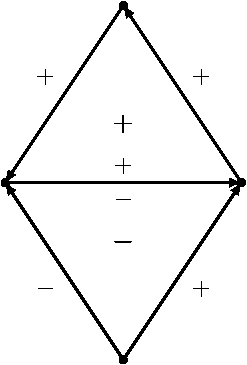
\includegraphics[width=.9\textwidth]{bilder/tikz/LBDEC.pdf}
      \end{minipage}\hfill
      \begin{minipage}[htp]{.7\textwidth}
        \centering
        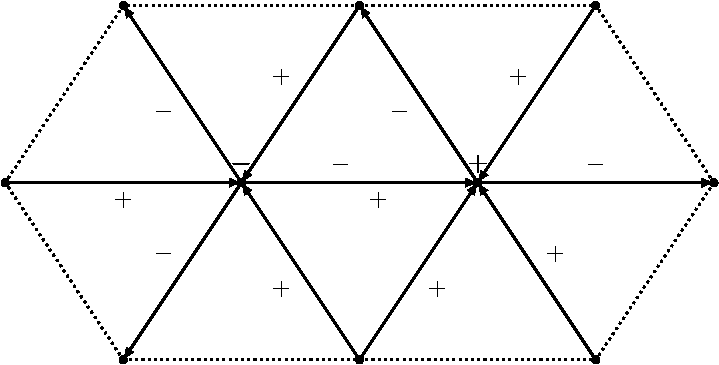
\includegraphics[width=.9\textwidth]{bilder/tikz/LCBDEC.pdf}
      \end{minipage}
      \caption{Signs \( s \) on example mesh extracts, which affected the discretization of the discrete Laplace operators.
               Left (\( \LBh \)): The edge of interest \( e \) is the middle edge.
                                  The bold signs in the middle of the faces indicate \( s_{f,e} \).
                                  The other signs at the local edges \( \tilde{e} \) (regarding the two faces \( f \)) indicate \( s_{f,\tilde{e}} \).
               Right (\( \LCBh \)): The edge of interest \( e \) is also the middle edge.
                                    The bold signs above the two inner vertices \( v \) indicate \( s_{v,e} \).
                                    The other signs at the local edges \( \tilde{e} \) (regarding the two vertices \( v \))
                                    indicate \( s_{v,\tilde{e}} \).}
       \label{figSigns}
    \end{figure}

  \subsection{Discrete norm}
    
    Approximating the norm \( \left\| \pfl \right\| \) on a edge \( e\in\E \) is not so easy like the development of discrete linear
    operators. 
    We only know how \( \pflh \) "act" on a single edge, so \( \pflh \) gives us only one dimensional informations.
    In other words, we only know the proportion \( \ph \cdot \e = \pflh (e)\) of the discrete contravariant vector field 
    \( \ph = \left( \pflh \right)^{\sharp} \) in the
    \( \e \) direction, but we don't know the length of \( \ph \) defined on this edge.

    ...maybe some averaging techniques, which I tried and why these sucks...
   
    One way out is to rise the dimension of the discrete 1-forms, therefor we introduce some bases at the intersection 
    \( c(e) = e\cap (\star e) \) of a edge and its dual edge to describe discrete contra- and covariant vector fields in a local 
    (piecewise flat)
    coordinate system.

    The basis for contravariant vectors at \( c(e) \) is composed of
    \begin{align}
      \partial_{e}X &:= \e = \v_{2} - \v_{1} \\
      \partial_{\star e}X &:= *\e =  c(f_{2}) - c(f_{1})
    \end{align}
    if \( e=\left[ v_{1}, v_{2} \right] \) and the face \( f_{1} \) lay right and \( f_{2} \) left of \( e \) (...figure...). 
    This definitions are consistent with the canonical basis, if the position \( X \) is a barycentric parametrisation of the edge \( e \)
    resp. its dual, i.e. for
    \begin{align}
      X_{e}(t_{e}) &= t_{e}\v_{2} + \left( 1 - t_{e} \right)\v_{2} \text{ for } t\in[0,1]\\
      X_{\star e}(t_{\star e}) &=\begin{cases}
                        2t_{\star e}c(e) + \left( 1 - 2t_{\star e} \right) c(f_{1}) & \text{if } t_{\star e}\in\left[ 0 , \frac{1}{2} \right] \\
                        \left(1 - t_{\star e}\right) c(e) + \left( 2t_{\star e} - 1 \right) c(f_{1}) 
                                & \text{if } t_{\star e}\in \left[\frac{1}{2} , 1\right]
                      \end{cases}
    \end{align}
    holds \( \partial_{e}X = \partial_{t_{e}}X_{e} \) 
    and \( \partial_{\star e}X = \frac{1}{2} \left( \partial_{t_{\star e}}X_{\star e}|_{\left[ 0 , \frac{1}{2} \right]} 
                                                   + \partial_{t_{\star e}}X_{\star e}|_{\left[\frac{1}{2}, 1 \right]}\right) \).
    Therefore we get the local metric tensor
    \begin{align}
      \mathbf{g}_h(e) &= \left| e \right|^{2} \left( dx^{e} \right)^{2} + \left| \star e \right|^{2} \left( dx^{\star e} \right)^{2}
    \end{align}
    where \( \left\{  dx^{e}, dx^{\star e} \right\} \) are the dual base of \( \left\{ \partial_{e}X, \partial_{\star e}X \right\} \),
    i.e. \( dx^{i}\left(\partial_{j}X\right) = \delta^{i}_{j} \) for \( i,j\in\left\{ e, \star e \right\} \).
    This gives us the great possibility to define
    \begin{align}
      \PDpflh(e) &:= \pflh(e)dx^{e} + \pflh(\star e)  dx^{\star e} 
                   = \pflh(e)dx^{e} - \frac{\left| \star e \right|}{\left| e \right|} \left(*\pflh\right)(e)  dx^{\star e} \\
                 &=  \pflh(e)\PDxi^{e} + \left(*\pflh\right)(e)\PDxi^{\star e}
                 =:
                   \begin{bmatrix}
                     \pflh \\ *\pflh 
                   \end{bmatrix}_{\text{PD}} (e)
    \end{align}
    where \( \PDxi^{e}:=dx^{e} \) and \( \PDxi^{\star e}:= - \frac{\left| \star e \right|}{\left| e \right|}dx^{\star e}\) are the
    contravariant Primal-Dual-basis (PD-basis), which we want to use.
    \( \PDpflh(e) \) is called the discrete Primal-Dual-1-form (PD-1-form).
    With this scaling and the condition \( \PDxi_{i}(\PDxi^{j}) = \delta^{j}_{i} \), 
    it is also possible to define the covariant PD-basis as 
    \( \PDxi_{e}:=\partial_{e}X \) and \( \PDxi_{\star e}:= -\frac{\left| e \right|}{\left| \star e \right|}\partial_{\star e}X \).
    Hence, we obtain for the discrete Primal-Dual-vector field (PD-vector field) \( \PDph \)
    \begin{align}
      \PDph(e) &:= \left(\PDpflh(e)\right)^{\sharp} 
                 = \frac{1}{\left| e \right|^{2}} \pflh(e)\partial_{e}X + \frac{1}{\left|\star e \right|^{2}} \pflh(\star e)\partial_{\star e}X \\
               &= \frac{1}{\left| e \right|^{2}} \pflh(e)\partial_{e}X 
                   -\frac{1}{\left| e \right|\left|\star e \right|} \left(*\pflh\right)(e) \partial_{\star e}X \\
               &= \frac{1}{\left| e \right|^{2}}\left[ \pflh(e)\PDxi_{e} + \left(*\pflh\right)(e)\PDxi_{\star e} \right]
               =: \begin{bmatrix}
                     \pflh \\ *\pflh 
                   \end{bmatrix}^{\text{PD}} (e)
    \end{align}
    Hence, we get for the square of the norm on \( c(e) \) 
    (and also with a constant interpolation on the whole edge) by contract the PD-1-Form with its corresponding PD-Vector
    \begin{align}
      \left\| \PDpflh \right\|_{h}^{2}(e) := \left( \PDpflh\left( \PDph \right) \right)(e)
                                       = \frac{1}{\left| e \right|^{2}}\left( \left[ \pflh(e) \right]^{2} 
                                                                             +\left[ \left(*\pflh\right)(e) \right]^{2}\right)
    \end{align}
    In general, we also get a local discrete inner product between \( \PDpflh \) and another PD-1-form \( \PDqflh \) by
    \begin{align}
      \left\langle \PDqflh , \PDpflh \right\rangle_{h}(e)
          &:= \left( \PDqflh\left( \PDph \right) \right)(e)
                                       = \frac{1}{\left| e \right|^{2}}\left( \left[\pflh\qflh\right](e) 
                                                                             +\left[\left(*\pflh\right)\left(*\qflh\right)\right](e) \right)
    \end{align}
    or a outer product between the PD-1-form \( \PDpflh \) and the PD-vector  \( \PDqh \) to produce the PD-(1,1)-Tensor
    \begin{align}
      \left(\PDpflh \otimes \PDqh\right) 
          &:= \frac{1}{\left| e \right|^{2}} \left( \pflh\qflh \PDxi^{e}\otimes\PDxi_{e} 
                                                   +\pflh(*\qflh) \PDxi^{e}\otimes\PDxi_{\star e}
                                                   +(*\pflh)\qflh \PDxi^{\star e}\otimes\PDxi_{e}
                                                   +(*\pflh)(*\qflh)\PDxi^{\star e}\otimes\PDxi_{\star e}\right)\\
          &=: \frac{1}{\left| e \right|^{2}} 
            \begin{bmatrix}
              \pflh\qflh & \pflh(*\qflh) \\
              (*\pflh)\qflh & (*\pflh)(*\qflh)
            \end{bmatrix}^{D}_{P} 
    \end{align}
    (Arguments \( (e) \) are omitted)


\section{Discrete PD-Problem, a DEC approach}
  To use a PD-1-form solution, we must also determine the dual part \( *\pflh \), 
  therefore we discretize the Hodge dual equation \eqref{eqDOC} (resp. \eqref{eqD}) simultaneous to the primal equation
  \eqref{eqPOC} (resp. \eqref{eqP}).
  This leads to the DEC-discretized Primal-Dual-problem (DEC-PD-problem) 
  \begin{align}
    \left[ \partial_{t} + K_{0}\LDRh + K_{n}\left( \left\| \PDpflh \right\|_{h}^{2} - 1 \right) \right]\PDpflh &= 0
  \end{align}
  respective, without the One-Constant-Approximation,  
  \begin{align}
    \left[ \partial_{t} -   
            \begin{bmatrix}
               K_{1} \\ K_{3}
            \end{bmatrix} \LCBh
            -\begin{bmatrix}
               K_{3} \\ K_{1}
            \end{bmatrix} \LBh
    + K_{n}\left( \left\| \PDpflh \right\|_{h}^{2} - 1 \right) \right]\PDpflh &= 0
  \end{align}

  \subsection{Time discretization}
    The simplest way to discretize the DEC-PD-problem in time is to use a implicit Euler scheme, 
    where we handle the norm \( \left\| \PDpflh \right\|_{h}^{2} \) explicit.
    For one Euler step, we have to solve
    \begin{align}
      \left[ \frac{1}{\tau} + K_{0}\LDRh + K_{n}\left( \left\| \PDpflhOld \right\|_{h}^{2}(e) - 1 \right) \right]\PDpflh(e) 
          &= \frac{1}{\tau} \PDpflhOld(e)
    \end{align}
    resp.
    \begin{align}
       \left[  \frac{1}{\tau}-   
            \begin{bmatrix}
               K_{1} \\ K_{3}
            \end{bmatrix} \LCBh
            -\begin{bmatrix}
               K_{3} \\ K_{1}
            \end{bmatrix} \LBh
    + K_{n}\left( \left\| \PDpflhOld \right\|_{h}^{2}(e) - 1 \right) \right]\PDpflh(e) 
          &= \frac{1}{\tau} \PDpflhOld(e)
    \end{align}
    for all \( e\in\E \).
    \( \PDpflhOld  \) is the solution of the last time step or the initial condition, if this is the first Euler step.
    \( \tau = t - \hat{t}  \) is the time step wide.
    
    The drawback of this semi-implicit Euler scheme is, that we need very small \( \tau \).
    Therefore, it is better to use a Taylor-linearisation for  \( \left\| \PDpflh \right\|_{h}^{2}\PDpflh \).
    First we calculate the partially component derivative on a edge \( e\in\E \) of
    \begin{align}
        \Phi\left( \PDpflh \right) &= \Phi \left( \pflh, *\pflh \right)
              :=\left\| \PDpflh \right\|_{h}^{2}\PDpflh 
              = \frac{1}{\left| e \right|^{2}} \left( \left( \pflh \right)^{2} 
                                                  +\left( *\pflh \right)^{2} \right)
                                     \begin{bmatrix}
                                       \pflh \\ *\pflh
                                     \end{bmatrix}
    \end{align}
    (Henceforward, for a better readability, the arguments \( e \) are omitted).
    Hence, we obtain
    \begin{align}
      \partial_{\pflh}\Phi
          &= \frac{1}{\left| e \right|^{2}}
                \begin{bmatrix}
                  3\left( \pflh \right)^{2} + \left( *\pflh \right)^{2} \\
                  2\pflh\left( *\pflh \right)
                \end{bmatrix} \\
      \partial_{*\pflh}\Phi
          &= \frac{1}{\left| e \right|^{2}}
                \begin{bmatrix}
                  2\pflh\left( *\pflh \right) \\
                  \left( \pflh \right)^{2} + 3 \left( *\pflh \right)^{2} \\
                \end{bmatrix}
    \end{align}
    For one step Taylor at \( \PDpflhOld \), we get
    \begin{align}
      \Phi(\PDpflh) &\approx  \Phi(\PDpflhOld) + \left( \pflh - \pflhOld \right)\partial_{\pflh}\Phi\left( \PDpflhOld \right)
                          + \left( *\pflh - *\pflhOld \right)\partial_{*\pflh}\Phi\left( \PDpflhOld \right) \\
                    &= \left\| \PDpflhOld \right\|_{h}^{2}\PDpflhOld
                    +\frac{1}{\left| e \right|^{2}}
                      \begin{bmatrix}
                        \left( \pflh - \pflhOld \right)\left( 3\left( \pflh \right)^{2} + \left( *\pflh \right)^{2} \right)
                        + 2\left(*\pflh - *\pflhOld\right)\pflh\left( *\pflh \right) \\
                        2\left( \pflh - \pflhOld \right)\pflh\left( *\pflh \right)
                        +\left(*\pflh - *\pflhOld\right)\left( 3\left( \pflh \right)^{2} + \left( *\pflh \right)^{2} \right)
                      \end{bmatrix} \\
       &= \left\| \PDpflhOld \right\|_{h}^{2}\PDpflhOld
          \begin{aligned}[t]
            &-\frac{3}{\left| e \right|^{2}}\left( \left( \pflhOld \right)^{2} + \left( *\pflhOld \right)^{2} \right)\PDpflhOld
            +\frac{2}{\left| e \right|^{2}}
                    \begin{bmatrix}
                      \left( *\pflhOld \right)^{2} \\  \left( \pflhOld \right)^{2}
                    \end{bmatrix}
                    \PDpflhOld \\
            &+\frac{1}{\left| e \right|^{2}}\left( \left( \pflhOld \right)^{2} + \left( *\pflhOld \right)^{2} \right)\PDpflh
            +\frac{2}{\left| e \right|^{2}}
                    \begin{bmatrix}
                      \pflh\pflhOld \\ \left( *\pflh \right)\left( *\pflhOld \right)
                    \end{bmatrix}
                    \PDpflhOld \\
            &+\frac{2}{\left| e \right|^{2}}
                \begin{bmatrix}
                  \left(*\pflh - *\pflhOld\right)\left( *\pflh \right)\\
                  \left( \pflh - \pflhOld \right)\pflh
                \end{bmatrix}
                \PDpflhOld
          \end{aligned}\\
       &= -2\left\| \PDpflhOld \right\|_{h}^{2}\PDpflhOld 
            + \left\| \PDpflhOld \right\|_{h}^{2}\PDpflh
            + 2\left\langle \PDpflh, \PDpflhOld \right\rangle_{h}\PDpflhOld
    \end{align}
    The inner product term can be also expressed as matrix-vector multiplication:
    \begin{align}
      \left\langle \PDpflh, \PDpflhOld \right\rangle_{h}\PDpflhOld
        = \frac{1}{\left| e \right|^{2}}
            \begin{bmatrix}
              \left( \pflhOld \right)^{2} & \pflhOld\left( *\pflhOld  \right) \\
              \pflhOld\left( *\pflhOld  \right) & \left( * \pflhOld \right)^{2}
            \end{bmatrix}_{P}^{D} \cdot \PDpflh
        = \left( \PDpflhOld \otimes \PDphOld \right) \cdot \PDpflh
    \end{align}

    With the Taylor linearization and the implicit Euler scheme, we have to solve the following PD-DEC-Problem in every time steps and all \( e\in\E \)
    \begin{align}
      \left[ \frac{1}{\tau} + K_{0}\LDRh + K_{n}\left( \left\| \PDpflhOld \right\|_{h}^{2} - 1 \right) \right]\PDpflh
          + 2K_{n} \left( \PDpflhOld \otimes \PDphOld \right) \cdot \PDpflh
          &= \left[\frac{1}{\tau} + 2K_{n}\left\| \PDpflhOld \right\|_{h}^{2}\right]\PDpflhOld
    \end{align}
    resp.
    %\resizebox{0.9\textwidth}{!}{\begin{minipage}{\linewidth}
    \begin{align} 
      \left[ \frac{1}{\tau}
          - \begin{bmatrix}
               K_{1} \\ K_{3}
            \end{bmatrix} \LCBh
            -\begin{bmatrix}
               K_{3} \\ K_{1}
            \end{bmatrix} \LBh
          + K_{n}\left( \left\| \PDpflhOld \right\|_{h}^{2} - 1 \right) \right]\PDpflh
          + 2K_{n} \left( \PDpflhOld \otimes \PDphOld \right) \cdot \PDpflh
          &= \left[\frac{1}{\tau} + 2K_{n}\left\| \PDpflhOld \right\|_{h}^{2}\right]\PDpflhOld
    \end{align}
    %\end{minipage}}

    
\section{Notes on Implementation}

  \subsection{Edge mesh}

    \subsubsection{Iterators}

  \subsection{Matrix assembling}

  \subsection{Sharp and flat interpolations}



  

\bibliography{bibl}
\bibliographystyle{alpha}

\end{document}
